%% Преамбула TeX-файла

% 1. Стиль и язык
\documentclass{G7-32} % Стиль (по умолчанию размер шрифта 14pt)

% Остальные стандартные настройки убраны в preamble.inc.tex.
\sloppy

% Настройки стиля ГОСТ 7-32
% Для начала определяем, хотим мы или нет, чтобы рисунки и таблицы нумеровались в пределах раздела, или нам нужна сквозная нумерация.
\EqInChapter % формулы будут нумероваться в пределах раздела
\TableInChapter % таблицы будут нумероваться в пределах раздела
\PicInChapter % рисунки будут нумероваться в пределах раздела

% Добавляем гипертекстовое оглавление в PDF
\usepackage[
bookmarks=true, colorlinks=true, unicode=true,
urlcolor=black,linkcolor=black, anchorcolor=black,
citecolor=black, menucolor=black, filecolor=black,
]{hyperref}

\AfterHyperrefFix

\usepackage{microtype}% полезный пакет для микротипографии, увы под xelatex мало чего умеет, но под pdflatex хорошо улучшает читаемость

% Тире могут быть невидимы в Adobe Reader
\ifInvisibleDashes
\MakeDashesBold
\fi

\usepackage{graphicx}   % Пакет для включения рисунков

% С такими оно полями оно работает по-умолчанию:
% \RequirePackage[left=20mm,right=10mm,top=20mm,bottom=20mm,headsep=0pt,includefoot]{geometry}
% Если вас тошнит от поля в 10мм --- увеличивайте до 20-ти, ну и про переплёт не забывайте:
\geometry{right=20mm}
\geometry{left=30mm}
\geometry{bottom=20mm}
\geometry{ignorefoot}% считать от нижней границы текста


% Пакет Tikz
\usepackage{tikz}
\usetikzlibrary{arrows,positioning,shadows}

% Произвольная нумерация списков.
\usepackage{enumerate}

% ячейки в несколько строчек
\usepackage{multirow}

% itemize внутри tabular
\usepackage{paralist,array}

%\setlength{\parskip}{1ex plus0.5ex minus0.5ex} % разрыв между абзацами
\setlength{\parskip}{1ex} % разрыв между абзацами
\usepackage{blindtext}

% Центрирование подписей к плавающим окружениям
%\usepackage[justification=centering]{caption}

\usepackage{newfloat}
\DeclareFloatingEnvironment[
placement={!ht},
name=Equation
]{eqndescNoIndent}
\edef\fixEqndesc{\noexpand\setlength{\noexpand\parindent}{\the\parindent}\noexpand\setlength{\noexpand\parskip}{\the\parskip}}
\newenvironment{eqndesc}[1][!ht]{%
    \begin{eqndescNoIndent}[#1]%
\fixEqndesc%
}
{\end{eqndescNoIndent}}



% Настройки листингов.
\ifPDFTeX
% 8 Листинги

\usepackage{listings}
\usepackage{float}

% Значения по умолчанию
\lstset{
  basicstyle= \footnotesize,
  breakatwhitespace=true,% разрыв строк только на whitespacce
  breaklines=true,       % переносить длинные строки
%   captionpos=b,          % подписи снизу -- вроде не надо
  inputencoding=utf-8,
  numbers=left,          % нумерация слева
  numberstyle=\footnotesize,
  showspaces=false,      % показывать пробелы подчеркиваниями -- идиотизм 70-х годов
  showstringspaces=false,
  showtabs=false,        % и табы тоже
  stepnumber=1,
  tabsize=4,              % кому нужны табы по 8 символов?
  frame=single
}

% Стиль для псевдокода: строчки обычно короткие, поэтому размер шрифта побольше
\lstdefinestyle{pseudocode}{
  basicstyle=\small,
  keywordstyle=\color{black}\bfseries\underbar,
  language=Pseudocode,
  numberstyle=\footnotesize,
  commentstyle=\footnotesize\it
}

% Стиль для обычного кода: маленький шрифт
\lstdefinestyle{realcode}{
  basicstyle=\scriptsize,
  numberstyle=\footnotesize
}

% Стиль для коротких кусков обычного кода: средний шрифт
\lstdefinestyle{simplecode}{
  basicstyle=\footnotesize,
  numberstyle=\footnotesize
}

% Стиль для BNF
\lstdefinestyle{grammar}{
  basicstyle=\footnotesize,
  numberstyle=\footnotesize,
  stringstyle=\bfseries\ttfamily,
  language=BNF
}

% Определим свой язык для написания псевдокодов на основе Python
\lstdefinelanguage[]{Pseudocode}[]{Python}{
  morekeywords={each,empty,wait,do},% ключевые слова добавлять сюда
  morecomment=[s]{\{}{\}},% комменты {а-ля Pascal} смотрятся нагляднее
  literate=% а сюда добавлять операторы, которые хотите отображать как мат. символы
    {->}{\ensuremath{$\rightarrow$}~}2%
    {<-}{\ensuremath{$\leftarrow$}~}2%
    {:=}{\ensuremath{$\leftarrow$}~}2%
    {<--}{\ensuremath{$\Longleftarrow$}~}2%
}[keywords,comments]

% Свой язык для задания грамматик в BNF
\lstdefinelanguage[]{BNF}[]{}{
  morekeywords={},
  morecomment=[s]{@}{@},
  morestring=[b]",%
  literate=%
    {->}{\ensuremath{$\rightarrow$}~}2%
    {*}{\ensuremath{$^*$}~}2%
    {+}{\ensuremath{$^+$}~}2%
    {|}{\ensuremath{$|$}~}2%
}[keywords,comments,strings]

% Подписи к листингам на русском языке.
\renewcommand\lstlistingname{Листинг}
\renewcommand\lstlistlistingname{Листинги}

\else
\usepackage{local-minted}
\fi

% Полезные макросы листингов.
\include{macros.inc}

% Стиль титульного листа и заголовки
\include{00-title}


\begin{document}

\frontmatter % выключает нумерацию ВСЕГО; здесь начинаются ненумерованные главы: реферат, введение, глоссарий, сокращения и прочее.

%% \maketitle %создает титульную страницу


%% \begin{executors}
%% \personalSignature{Первый исполнитель}{ФИО}

%% \personalSignature{Второй исполнитель}{ФИО}
%% \end{executors}


\listoffigures                         % Список рисунков

\listoftables                          % Список таблиц

%\NormRefs % Нормативные ссылки 
% Команды \breakingbeforechapters и \nonbreakingbeforechapters
% управляют разрывом страницы перед главами.
% По-умолчанию страница разрывается.

% \nobreakingbeforechapters
% \breakingbeforechapters

% Также можно использовать \Referat, как в оригинале
\begin{abstract}

    Пояснительная записка содержит \pageref{LastPage}\,стр.%
    \ifnum \totfig >0
    , \totfig~рис.%
    \fi
    \ifnum \tottab >0
    , \tottab~табл.%
    \fi
    %
    \ifnum \totbib >0
    , \totbib~источн.%
    \fi
    %
    \ifnum \totapp >0
    , \totapp~прил.%
    \else
    .%
    \fi

        

\end{abstract}

%%% Local Variables: 
%%% mode: latex
%%% TeX-master: "rpz"
%%% End: 


\tableofcontents

\printnomenclature % Автоматический список сокращений

\Introduction

Особенностью современной индустрии разработки программного обеспечения является применение нескольких языков программирования в
одном программном проекте. Данная особенность порождает проблему проверки согласованности фрагментов кода, реализованных на разных языках и
применяемых в составе одной программной системы. Как правило, такая несогласованность отслеживается только на этапе отладки или тестирования.

Одним из вариантов решения данной проблемы может стать проведение статического семантического анализа кода
с выявлением несогласованности в таком коде автоматически. Для решения такого рода задач существуют различные
инструментальные средства и часто такие средства встраиваются в среду разработки для
поддержки разработчика в реальном времени.

Однако, на данный момент методы проведения статического анализа мультиязыкового
кода развиты слабо. Большая часть методов ориентирована на специфические языки или проекты
и плохо подходит для интеграции в инструментальные средства в общем случае.
Вследствие этого мультиязыковые средства поддержки разработчика слабо развиты
и обычно ограничены кругом узкоспециализированных проприетарных решений.

Метод мультиязыкового анализа, позволяющий гибко анализировать
фрагменты кода на разных языках и независимый относительно анализируемых
технологий является одним из решений данной проблемы.

\textbf{Актуальность темы исследования} обусловлена малым развитием
инструментальных средств поддержки разработчика, ориентированных на мультиязыковой анализ.
Такое положение вещей снижает продуктивность разработчиков и увеличивает время, отводимое
на процессы кодирования и отладки.

\textbf{Объектом исследования} являются исходные тексты и семантические модели
программ, написанных с использованием нескольких языков
программирования.

\textbf{Предметом исследования} являются методы и алгоритмы анализа исходных
текстов программ, ориентированных на мультиязыковой статический анализ.

\textbf{Целью работы} является упрощение процессов разработки ПО, путем создания метода выявления межъязыковых связей,
позволяющего обеспечивать корректность и расширяемость соответствующих средств.

Для достижения данной цели необходимо решить следующие \textbf{задачи}:
\begin{enumerate}[1)]
    \item изучить предметную область, а именно индустрию разработки ПО,
    \item провести исследование текущих решений в области межъязыкового анализа,
    \item разработать требования к методу и спроектировать его архитектуру,
    \item описать прикладные сценарии использования метода и соответствующего анализатора,
    \item создать первичную реализацию анализатора, поддерживающего определенный набор языков,
    \item провести оценку показателей анализатора на избранных тестовых проектах.
\end{enumerate}

\textbf{Научная новизна} работы заключается в создании метода анализа, позволяющего
разрабатывать различные инструментальные средства, направленные
на поддержку разработчика в процессе кодирования и отладки. При этом, такой метод позволит
обеспечить корректность семантического анализа на межъязыковом уровне.

\textbf{Практическая значимость} работы выражается в создании прототипа мультиязыкового
анализатора, обеспечивающего поддержку реализации сценариев LSP, что позволяет
создавать <<мультиязыковые>> серверы LSP.

\Define{Семантика}{смысловое содержание синтаксических конструкций программ}

\mainmatter % это включает нумерацию глав и секций в документе ниже

\chapter{Исследование существующих технологий и языков программирования в контексте
областей разработки программного обеспечения} \label{sec:num1}

\section{Современная индустрия разработки программного обеспечения}

Современные программные проекты, в отличие от многих программных проектов прошлого,
гораздо чаще состоят из набора разных (порой разительно) технологических
решений, предназначенных для решения определенного круга задач. Согласно \cite{empirical-analysis},
в одном программном проекте в среднем задействовано 5 языков программирования, один из
которых является <<основным>>, а остальные -- специализированными языками предметной области (DSL\Abbrev{DSL}{domain specific language ""--- язык разработанный для определенной предметной области}).
В заключении статьи авторы признают популярность мультиязыковых программных проектов
и оценивают важность наличия соответствующих инструментальных средств для работы с
такого рода проектами.

Также, нередко использование нескольких языков и в индустрии разработки. Так, авторы \cite{professional-developers}
провели исследование популярности мультиязыковых проектов
в результате опроса 139 профессиональных разработчиков из разных сфер. 
Результаты опроса показали, что опрашиваемые имели дело с 7 различными языками, в среднем.
При этом, в работу было вовлечено в среднем 3 пары связанных языков в контексте одного проекта.
Более 90\% опрашиваемых также сообщали о проблемах согласованности между языками,
встречаемых при разработке в такой мультиязыковой среде. 

Таким образом, в современной разработке программного обеспечения нередко использование
нескольких языков вне зависимости от объемов проекта или вовлекаемой предметной области.
Ситуация становится сложнее со временем, так как создание новых технологий разработки
часто влечет за собой формирование определенной нотации или языка для управления или конфигурации.
Например, это может касаться таких повсеместных технологий как СУБД\Define{СУБД}{система управления базами данных}, систем сборки,
серверов приложений или скриптов развертывания.

Для наглядности, можно привести следующие языки, нередко фигурирующие в составе современных программных проектов:
\begin{itemize}    
    \item язык разметки HTML в составе проекта, использующего ASP фреймворк,
    \item язык скриптов командной строки в составе проекта, использующего язык C,
    \item язык запросов SQL в составе проекта, использующего Python и фреймворк Flask,
    \item язык препроцессора в составе файла исходного кода, реализованного на C++.
\end{itemize}

Заключительный пункт списка примеров приведен для того, чтобы показать характер
связи различных технологий -- разным языкам необязательно даже находится в раздельных
файлах или модулях, нередки случаи полноценного переплетения различных синтаксисов и
семантик.

\subsection{Актуальность мультиязыкового статического анализа}

Итак, мультиязыковые программные проекты нередки. Следовательно, имеет смысл использования
различных техник работы с исходным кодом таких проектов, поддерживающих процесс разработки.
Одной из таких техник является статический анализ исходного кода. Его основной сценарий
использования это упрощение различных сценариев процесса разработки ПО -- кодирования,
верификации, рефакторинга и других.

Стоит уточнить что имеется под определением <<статический анализ кода>>. Статический
анализ это прежде всего набор различных техник по извлечению информации о программе без её
явного запуска \cite{static-program-analysis}. Таким образом, статический анализ может
быть полезен в сценариях, которые не предполагают явного запуска программы -- в сущности во
всех сценариях процесса разработки ПО исключая этапы тестирования и запуска.

Возможные сценарии использования статического анализа кода включают (но не ограничиваются):
\begin{itemize}
    \item оптимизацию программ во время компиляции,
    \item выявление потенциальных уязвимостей,
    \item доказательство сохранения определенных инвариантов,
    \item сбор определенной статистики,
    \item выявление <<пахнущих>> фрагментов кода,
    \item извлечение информации для помощи разработчику во время кодирования (линтинг),
    \item автоматический рефакторинг кода.
\end{itemize}

Так как сценарии использования статического анализа настолько разнообразны, в рамках данной работы
решено было сосредоточится на сценариях разработки, которые помогают в процессе кодирования и поддержки проекта.
Существуют различные инструментальные средства, способные упрощать такие сценарии.
К таким средствам, к примеру, относятся:
\begin{itemize}
    \item интегрированные средства разработки (IDE\Abbrev{IDE}{integrated development environment --- интегрированная среда разработки}),
    \item линтеры (собирательное название инструментов, первым из которых был <<Lint>> \cite{Johnson1978LintAC}),
    \item инструменты автоматического рефакторинга,
    \item инструменты сбора статистики,
    \item различные кодогенераторы и фреймворки \cite{qt-moc}\cite{react}.
\end{itemize}

Необходимость в таких средствах присутствует и она достаточно высока. Так, согласно
исследованию \cite{aid-developers}, использование средств поддержки разработчика
(в данной работе это механизмы анализа и навигации по межъязыковым связям) позволяет
улучшить как скорость разработки ПО, так и уменьшить количество совершаемых ошибок. Стоит заметить,
что несмотря на количество времени, прошедшее с момента проведения исследования, 
принципы разработки ПО в данной предметной области (веб-разработка) не изменились и большинство
программных проектов веб-приложений состоят как минимум из двух языков. 
Обычно это разделение проводится по принципу фронтенд и бекенд.

Согласно обзорной статье об исследовании межъязыковых связей \cite{pragmatic-evidence}, современные средства межъязыкового
и мультиязыкового анализа остаются всё еще плохо развитыми. Особенно это касается отношения корректности
таких средств. Более того, большая их часть часто является частным решением, ориентированным на определенную
предметную область или технологию, что снижает универсальность таких средств и усложняет их интеграцию.

Так как статья содержит большую выборку литературы по обнаружению и анализу межъязыковых связей, авторам удается
установить широкую область применения межъязыкового анализа. В эту область входят такие дисциплины разработки ПО как:
\begin{itemize}
    \item семантическое понимание программ,
    \item представление знаний при сопровождении систем,
    \item рефакторинг,
    \item моделирование ПО,
    \item валидация и верификация систем,
    \item визуализация систем,
    \item сбор статистик и метрик.
\end{itemize}

Как видно из списка, большинство этих дисциплин значительно пересекаются со сценариями использования
статического анализа кода, что говорит о том что реализация такого анализа может быть очень актуальной
для обеспечения упрощения и удешевления большого количества этапов разработки ПО.

\section{Особенности мультиязыкового анализа} \label{ssec:num1}

Мультиязыковой анализ вовлекает множество особенностей существующих инструментов, так как косвенно или
непосредственно семантическая информация об этих инструментах должна быть вовлечена в процесс анализа.
Поэтому стоит рассмотреть особенности мультиязыкового анализа которые затрудняют разработку соответствующих
анализаторов и процесс анализа в целом.

\subsection{Сложности распознавания текста} \label{ssec:parsing-problem}

Так как вовлекаемые фрагменты кода написаны на разных языках, проблема анализа таких фрагментов
возникает уже на самом первом этапе -- этапе распознавания текста. Обычно процесс анализа
текста с определенной грамматикой не вызывает труда так как грамматика фиксирована и анализатор строится
стандартными средствами -- парсер генераторы, рекурсивный спуск и иные. 

Однако, в случае парсинга текста на нескольких языках возникают сложности, так как создание универсальной
грамматики (для всех анализируемых языков) обычно трудоемко и порой в целом невозможно. Таким образом остается
несколько способов распознавания текста:
\begin{enumerate}[1)]
    \item распознавание и анализ текстов по отдельности,
    \item использование смешанных парсеров (например с использованием островных грамматик \cite{island-grammars}),
    \item использование единого представления для унификации различных парсеров.
\end{enumerate}

Первый пункт является простым в реализации и работает в большинстве случаев, однако
возникают сложности при анализе единого фрагмента (например, файла), который вовлекает несколько
языков в анализ (к примеру CSS стили в заголовке страницы HTML). Также, такой подход не позволяет
проводить совместный анализ и выявлять связи между модулями, реализованными на разных языках.

Второй пункт позволяет анализировать в том числе смешанные грамматики, 
но сборка таких парсеров довольно трудоемка и ограничена поддержкой лишь определенного количества языков.

Таким образом, наиболее оптимальным является вариант распознавания при котором мультиязыковые фрагменты
изначально переводятся в единое представление (используя любой специфичный способ перевода, сохраняющий семантику), а
уже затем анализируются. В некоторых случаях такой подход является наиболее удобным так как
интересующая область анализа может вовлекать только специфическую часть информации, представленную в коде.
В таком случае, универсальное представление может быть создано с учетом только такой информации и
в результате получиться гораздо проще исходного языка. Это позволяет упростить анализатор и облегчить его
дальнейшую поддержку.

\subsection{Анализ и кодогенерация}

Несмотря на то, что кодогенерация является сложностью которую приходится учитывать и при обычном
статическом анализе, в мультиязыковых проектах эта сложность выходит на новый уровень.
Это происходит в первую очередь потому, что большое количество технологических решений, вовлекающих
разные языки используют разные подходы к кодогенерации и по разному её осуществляют.

Для понимания возможных проблем, рассмотрим следующий фрагмент кода на C++:

\begin{minted}[linenos=true]{cpp}
// function.h
#include <stdio.h>
template <typename T>
T f(T a) {
#ifdef SOMEBAR
    return a * 2;
#else
    return a + 2;
#endif
}

// main.cpp
#include "function.h"
int main()
{
#ifdef SOMEFOO
    printf("%f", f<float>(10));
#else
    printf("%d", f<int>(5));
#endif
    return 0;
}
\end{minted}

Представим что есть два файла, <<function.h>> и <<main.cpp>>. Фрагменты, соответствующие файлам, помечены
комментариями. При статическом анализе такого кода для определения того, какая версия функции в итоге будет
сгенерирована при компиляции необходимо сделать следующее:
\begin{enumerate}[1)]
    \item узнать какие значения принимают переменные среды при компиляции этих файлов,
    \item для каждого из таких значений сгенерировать возможную конфигурацию кода,
    \item проанализировать каждую конфигурацию и объединить результаты анализа.
\end{enumerate}

В отношении данного примера, возможных конфигураций будет четыре. В общем случае количество конфигураций
можно определить как мощность декартового произведения множеств значений вовлеченных переменных.
Нетрудно представить, что такое количество может быть достаточно большим, например при количестве переменных
равном 10 с учетом того что эти переменные принимают только 2 значения, количество конфигураций равно 1024.

Еще одной особенностью кодогенерации является частое вовлечение сторонних инструментов. В отличие от
примера приведенного выше, многие фреймворки различных технологических стеков полагаются на кодогенерацию во время
сборки проекта. Обычно эта кодогенерация вовлекает генерацию на уровне файлов. В данном случае статический анализ
не сможет обеспечить анализ сгенерированных файлов без использования одного из двух подходов:
\begin{itemize}
    \item запуск сборки и генерации во временной директории с последующей очисткой,
    \item абстрактная интерпретация команд генератора.
\end{itemize}

Первый подход может вызвать большие сложности если генерация имеет в зависимостях какое-либо
недоступное на момент анализа окружение. Примером может быть генерация <<файлов-определений>> для проекта,
который должен быть использован на конкретном встроенном устройстве. Такие файлы обычно являются
способом объединения конфигурации программного кода и информации для устройства. К примеру, таким файлом
является \texttt{c++config.h} который часто идет в поставке с избранным компилятором C++ и является
встроенным заголовочным файлом. Нетрудно представить, что такой файл может различаться от компилятора к
компилятору и даже от версии к версии, а также просто может не существовать, так как стандарт C++
не затрагивает встроенные определения. 
До момента размещения проекта в специализированном окружении, нет информации 
о том какого рода определения необходимо генерировать для анализа.
Такое часто происходит при разработке встроенных систем по разным причинам: количество конфигураций
устройств, упрощение процесса разработки, недоступность устройств и т.д.

Второй подход является более сложным в реализации, так как различные кодогенераторы и фреймворки редко
имеют исчерпывающую документацию по особенностям кодогенерации, поэтому кодирование такой информации
часто будет неполным. Более того, особенности кодогенерации могут быть особенностью реализации
определенного инструмента, что может поменяться со временем. Поэтому, практическая реализация
таких анализаторов это сложный процесс, требующий большого количества времени и поддержки.

\subsection{Формирование выборки для анализа}

На первый взгляд формирование выборки кажется тривиальной проблемой. При моноязыковом анализе она
решается использованием сторонних инструментов, позволяющих получить набор файлов для анализа.
Такую информацию могут предоставлять системы сборки или развертывания, в крайнем случае достаточно
поиска в файловой системе определенного множества файлов.

Однако, при вовлечении нескольких языков в проект, получение соответствующих файлов путем простого
поиска может быть неадекватным решением по следующим причинам:
\begin{itemize}
    \item компоновка проекта из отдельных, несвязанных проектов,
    \item сборка проекта зависящая от условий в текущем окружении,
    \item специфика компоновки файлов в единый модуль зависит от конкретного языка и может отличаться.
\end{itemize}

Соответственно, для успешной практической интеграции анализатора, способного проводить мультиязыковой анализ
необходимо обеспечить также поддержку внешних инструментов, позволяющих правильно выбирать файлы для
анализа основываясь на конфигурации операционного окружения проекта. Таким образом, анализ проекта
первым этапом обязан обеспечивать анализ \textit{операционного окружения} проекта. Такая особенность
сильно усложняет анализатор и накладывает ограничения на технологии с которыми он может работать, так
как операционное окружение в общем случае включает состояние всего компьютера: файловая система, переменные
среды или реестр, подключение к сети и т.д. 

В данной работе проблема выборки файлов для анализа
не рассматривается, так как она несущественна для формирования метода межъязыкового анализа, 
который независим от какого-либо анализатора, его использующего.

\subsection{Динамическая и неявная природа межъязыковых связей}

Многие семантически важные связи в реальных мультиязыковых проектах являются неявными. В большей части это применимо
к фреймворкам и системам сборки, так как порой семантическая информация распределена в разных местах проекта,
вовлекая при этом и системные зависимости \cite{professional-developers} \cite{external-dependencies}.

С точки зрения практической реализации, неявные связи являются усложняющим обстоятельством, но не
делающим анализ невозможным. К сожалению, то же нельзя сказать в отношении динамических связей. Под
динамическими связями понимаются связи, которые устанавливаются на определенном этапе исполнения кода.
Например, это может быть формирование строки в коде JavaScript, которая потом может быть использована чтобы
получить определенные теги HTML страницы.

Несмотря на наличие динамических связей в определенных языках, значительное множество языков общего назначения (GPL), \Abbrev{GPL}{general programming language --- язык общего назначения}
все же имеют статическую типизацию либо статическое время связывания идентификаторов, не вовлекающее процесс вычисления.
Это позволяет проводить эффективный статический анализ таких языков. Однако, в случае гетерогенных проектов наличие динамической
связи гораздо более распространено. Это связано с различными причинами, основная из которых, возможно,
связана с разнообразием связываемых между собой технологий. 

Например, очень частой динамической (но также вполне явной) связью является зависимость фрагмента от состояния ФС \Abbrev{ФС}{файловая система}. Это практически всегда встречается
в различных системах сборки -- скрипты сборки напрямую зависят от наличия некоторых файлов в системе и
при их отсутствии вынуждены прерывать исполнение сборки, порой после нескольких часов работы. Таким образом
тратятся как физические ресурсы, так и снижается продуктивность программиста, что может приводить к
ухудшению процесса разработки.

\subsection{Разнообразие парадигм программирования}

Как уже сказано в предыдущем подпункте, значительное множество GPL являются статически типизированными
либо имеют статическое время связывания идентификаторов. Однако, это касается по большей части
императивных языков программирования. Примерами могут служить Java, C\#, C++, Golang и другие.
Многие DSL однако, являются динамическими языками в том смысле, что они имеют позднее
связывание идентификаторов (обычно во время исполнения). Связано это в том числе с тем, что многие DSL
имеют другую парадигму программирования, что также влияет на особенность их реализации. Примерами могут служить 
языки сборки, языки командной оболочки или языки выборки данных (например, языки запросов к СУБД).

Многие фреймворки <<программируются>> не напрямую, а через конфигурационные файлы. Примером может служить
повсеместный язык разметки XML, который иногда эксплуатируется как язык описания каких-либо выражений на
определенном DSL. Ярким примером может служить система сборки Apache Ant, в ней узлы XML дерева
могут представлять обращения к переменным или даже целые выражения. Можно сказать, что любые конфигурационные
данные проекта могут представлять семантически важную информацию, так как использование конфигурационных
файлов в гетерогенных проектах повсеместно \cite{external-dependencies}.

Это приводит к тому, что некоторые вовлекаемые в анализ языки не являются языками программирования, но
всё же представляют семантическую ценность для анализа. Вследствие этого возникает проблема создания
метода такого анализа, который в том числе будет вовлекать такого рода фрагменты.

\subsection{Результаты исследования}

Подводя итоги раздела \ref{sec:num1}, можно сказать что современные проекты действительно
часто реализованы на различных языках, т.е. являются гетерогенными. Такой положение вещей
затрудняет многие сценарии разработки ПО и создание метода анализа обеспечивающего выявление межъязыковых
связей является хорошим способом решения многих возникающих проблем.

Также, на основе подпункта \ref{ssec:num1} можно выявить желаемые особенности метода мультиязыкового анализа:
\begin{enumerate}[1)]
    \item анализ с использованием единого представления является более эффективным решением ввиду большей универсальности,
    \item желательна поддержка сценариев кодогенерации, либо возможность их реализации,
    \item необходимо вовлечение операционного окружения проекта для обеспечения корректности анализа,
    \item эффективный анализ должен быть универсальным для многих языков и парадигм программирования.
\end{enumerate}

\clearpage
\chapter{Анализ состояния работ в области анализа мультиязыковых исходных текстов программ} \label{sec:num2}

\section{Теоретические и практические труды в отношении мультиязыкового анализа} \label{ssec:num2}

На данный момент область мультиязыкового анализа (в т.ч. не только статического) является
<<terra incognita>> -- в том смысле, что многие исследования на данную тему несут частный характер и не
имеют четко структурированной теоретической базы. Также, существуют концептуальные и онтологические сложности
в отношении этой области знаний. Например, для определения термина <<язык программирования>> в данной области
недостаточно рассматривать общепринятые варианты языков, так как чаще всего они являются GPL,
чего недостаточно в контексте мультиязыкового анализа. Термин <<формальный язык>> является более подходящим, но
сильно расширяет предметную область, что затрудняет создание единой терминологической базы.

Несмотря на данные сложности, работы по мультиязыковому анализу являются очень разнообразными и, рассмотрение
определенного количества таких работ позволит выявить общие аспекты анализа, которые универсальны для всех методов.
В данной работе была проведена выборка пяти различных работ по следующим показателям:
\begin{itemize}
    \item парадигма анализируемых языков,
    \item способ извлечения знаний (вовлекаемая онтологическая модель),
    \item вовлекаемые языки,
    \item сценарии использования анализаторов,
    \item возможные недостатки подхода.
\end{itemize}

\section{Pangea} \label{ssec:pangea}

Pangea \cite{pangea} это фреймворк для осуществления статического анализа, позволяющий
быстро разрабатывать различные анализаторы путем использования снимков системы (англ Object Model Snapshots).
Такие снимки являются исполняемыми образами моделей Moose \cite{moose}, которые в свою очередь получаются из
анализа исходного кода с использованием \textit{метамоделей} FAMIX \cite{famix}.

Фреймворк предназначен в первую очередь для анализа систем на основе определенных метрик,
которые в свою очередь собираются скриптом, реализованным на Smalltalk. В статье авторами показаны
различные сценарии использования фреймворка (в основном для Java приложений) -- сборка метрик и статистик,
с последующим анализом. Авторами заявляется поддержка других языков (C/C++, C\#, Smalltalk) путем использования других анализаторов,
предоставляющих результаты анализа в формате FAMIX.

Несмотря на то, что фреймворк может быть использован для многих языков, его средствами нельзя достичь именно
межъязыкового анализа, так как такой анализ подразумевает обработку межмодульных зависимостей, чего
данный фреймворк делать не позволяет. Также, одним из серьезных ограничений (в том числе замеченном авторами) является
ориентированность на OO \Abbrev{OO}{object oriented --- объектно ориентированный} языки, что ограничивает круг поддерживаемых языков.

Стоит заметить, что применение метамоделей на основе ОО парадигмы может затруднять
разработку соответствующих анализаторов. Основная причина этого -- понятия <<класс>> и <<объект>> являются довольно
размытыми семантически и их формальная реализация может разительно отличаться от языка к языку.
Основным примером такой сложности может служить сравнение языков JavaScript и Java. 

Несмотря на внешнюю схожесть, JavaScript куда больше напоминает сочетание Smalltalk и Scheme, что делает его более гибким
и, в каком-то отношении, функциональным языком. Отражение этого заключается к примеру в том, что до 
стандарта ES6 \cite{ecma262}, JavaScript считался чисто объектным языком и не содержал классов. Многие
<<классовые>> конструкции были реализованы через механизм прототипного наследования и обычные функции.
В случае Java класс является основопологающей конструкцией, основным блоком построения программ. В связи
с этим, многие семантические особенности Java (например, виртуальные вызовы или определения процедур) сильно
связаны с семантикой классов. К примеру, невозможно определить процедуру, без создания соответствующего класса.

В конце концов попытка объединения семантических понятий <<класс>> и <<объект>> сделает онтологическую модель
слишком сложной так как будет вовлекать абсолютно разные концепции из обоих языков. Решением данной проблемы
может стать использование <<меньшего>> унифицированного представления, т.е. сопровождающего
достаточное количество информации о сущности языка и при этом являющимся <<наибольшим общим делителем>>
среди различного набора языков.

\section{Статический анализ JNI связей} \label{ssec:jni}

JNI \cite{JNI} это набор API для взаимодействия виртуальной машины Java
с нативным кодом (к примеру, реализованным на C/C++ или ассемблере). Основная цель такого интерфейса --
доступ к низкоуровневым функциям, позволяющим ускорить исполнение кода на Java.

Как следует из описания, написание кода с использованием JNI влечет взаимодействие нескольких языков между
собой, в случае рассматриваемой статьи это Java и C++. В рамках статьи рассматривается статический анализ
на основе <<S-MLDA>>. Это разработанный авторами анализатор, позволяющий строить граф зависимостей вызовов 
(CDG) \Abbrev{CDG}{call-dependency graph --- граф зависимостей вызовов}
между фрагментами кода реализованными на двух языках. Процесс построения такого
графа заключается в парсинге и дальнейшем лексическом сравнении идентификаторов. В дальнейшем, такой
граф позволяет выявить связи компонентов и интерпретировать их должным образом (например, сообщить о 
несогласованности).

Основным недостатком метода является процесс лексического сравнения для реализации модели анализа.
Хотя и простой, такой метод является нестабильным и сложно поддерживаемым по следующим причинам:
\begin{itemize}
    \item имена идентификаторов неявно вовлекаются в процесс анализа семантики,
    \item возможны ложноположительные или ложноотрицательные результаты анализа при различном именовании,
    \item от версии к версии имена могут меняться, что сделает анализ менее полным.
\end{itemize}

Таким образом, метод анализа семантики посредством лексического сравнения является
довольно хрупким решением, поддерживающим малый набор языков. Также, такое решение является трудно поддерживаемым
и расширяемым в дальнейшем. 

Также стоит заметить что построение графа зависимостей вызовов является достаточно хорошим решением для многих
языков, так как широкий спектр межъязыкового взаимодействия может быть выражен через вызовы функций из одного
модуля в другом. С практической точки зрения такой подход является, пожалуй, наиболее простым в реализации, однако
такая модель сохраняет очень мало информации о семантике исходного языка, что затрудняет дальнейшее расширение
анализаторов на основе такой модели.

\section{MLSA} \label{ssec:mlsa}

MLSA (MultiLingual Software Analysis) \cite{MLSA} это метод, ориентированный на построение мультиязыковых анализаторов
путем организации определенного конвеера из анализаторов двух категорий -- языкозависимых и языконезависимых.
Используя исходное AST программы на определенном языке программирования, авторами предполагается
создание транслятора из такого AST в обобщенную форму (в статье такой транслятор называется <<interop фильтр>>),
а затем анализ такой обобщенной формы в контексте нескольких языков (такой анализатор называется <<MLSA фильтр>>).
Трансляторы являются языкозависимыми, а анализаторы языконезависимыми.

Также, стоит отметить, что авторами активно используется островная грамматика \cite{island-grammars} для
распознавания только интересующих фрагментов кода. Таким образом, сочетание различных фильтров и островная грамматика
в их основе создает гибкую и модульную систему при которой возможно создание различных анализаторов различной сложности.

Однако, основной проблемой данного подхода является рост числа необходимых анализаторов при увеличении
количества взаимодействующих языков. Допустим, при анализе 10 языков, взаимодействующих между собой, необходимо
будет создать 10 языкозависимых трансляторов и 50 языконезависимых анализаторов, организованных в виде
дерева. Конечно, такой случай является утрированным, однако как уже было сказано в разделе \ref{sec:num1}, в современном
программном проекте в среднем содержится 5 языков.

Данный метод как и предыдущий полагается на использование графа зависимостей вызовов, что сужает его применимость
в контексте языков, не имеющих функций (например форматы данных).

\section{Граф вызовов, семантики и номинальной схожести} \label{ssec:graphs}

В статье \cite{SNDGA} авторами решается проблема модуляризации мультиязыкового ПО путем построения специализированного графа
и анализа такого графа с использованием генетического алгоритма. В рамках данной работы интерес представляет
граф, использованный для отражения зависимостей в мультиязыковом коде.

В статье используется нестандартных композитный граф, состоящий из трех различных графов:
\begin{enumerate}[1)]
    \item граф зависимостей вызовов,
    \item граф семантических зависимостей,
    \item граф номинальной схожести.
\end{enumerate}
Все три графа имеют общую основу -- узлы представляют собой <<артефакты>>. Семантика ребер при этом зависит от типа графа.
Стоит разобрать каждый граф по отдельности.

Граф зависимостей вызовов представляет собой стандартный граф, встречаемый в других работах на данную тему. Ребра данного графа
представляют собой зависимость <<вызов>>, что в общем плане является зависимостью <<использует>>. В статье граф является взвешенным, что
позволяет авторам кодировать количество <<использований>> между артефактами как вес соответствующего ребра.
Построение графа зависимостей вызовов является языкозависимой процедурой и подразумевает использование соответствующего
анализатора для каждого вовлеченного языка.

Граф семантических зависимостей строится интересным образом. Авторами используется ВЛСА \Abbrev{ВЛСА}{вероятностный латентно-семантический анализ} для получения
значения схожести двух артефактов. Артефакты объединяются между собой и вес ребер в графе при этом соответствует схожести соединенных
узлов. Таким образом, метод построения графа является чисто лексическим и вовлекает статистические методы.

Граф номинальной схожести строится по похожему принципу что и предыдущий, однако в данном графе вес ребра отвечает не
за семантическую схожесть понятий, а за лексическую. Гипотеза авторов состоит в том, что осмысленно разработанные
системы часто имеют схожие назавания связанных между собой компонентов.

В итоге три таких графа объединяются и анализируются в дальнейшем генетическим алгоритмом. Данный граф
является интересной моделью представления информации так как позволяет сильно увеличить полноту анализа, пренебрегая
корректностью. Учитывая, что корректность анализа не требуется во всех сценариях использования статических анализаторов
(допустим как в случае работы авторов), такой подход выглядит действительно адекватным для определенного круга задач.
Также, как граф семантических зависимостей так и граф номинальной схожести не требуют языкозависимого анализатора для построения, что
сильно упрощает реализацию такого анализа на практике.

\section{Polycall} \label{ssec:polycall}

Статья \cite{polycall} интересна в первую очередь выбором онтологической модели. Вместо создания 
какой-либо модели на основе формальной спецификации, авторами предполагается использование
существующего формального языка с собственной семантикой. В случае данной статьи это язык WASM \cite{wasm}.
WASM является низкоуровневым языком программирования, ориентированным на встраивание в различные решения, в первую очередь 
браузеры.

В рамках данной статьи WASM рассматривается как <<наибольший общий делитель>>, который позволяет объединить
семантику различных языков путем простой компиляции из избранного языка в WASM модуль. Такой подход позволяет
сильно упростить процесс анализа, так как языкозависимым анализатором в данном случае выступает компилятор и
основная работа может заключаться в анализе непосредственного самих WASM модулей.

Несмотря на многообещающие особенности такого подхода, он имеет ряд недостатков. 

Во-первых, при компиляции в такое унифицированное представление теряется ряд типовой информации, так как обычно она не требуется для исполнения.
Это влечет за собой вероятную потерю основной информации, способной обеспечивать полноту анализа. 

Во-вторых, способ компоновки текстов исходного языка может отличаться от способа компоновки текстов языка унифицированного представления.
Одним из ярких примеров является процесс трансформации имен (англ. Name mangling) при компиляции кода C++. Это деталь реализации
компилятора, которая позволяет осуществлять перегрузку функций по типам принимаемых параметров. Впоследствии, при связывании
фрагментов C++, компилятор использует именно такие имена. Этот механизм мешает возможности связывания с скомпилированным кодом
другого языка, например в случае модулей реализованных на С. В связи с этим в C++ существует директива \texttt{extern "C"}.

В-третьих, многие языки в ходе компиляции подвергаются процессу ловеринга. Ловеринг это процесс переписывания изначальной программы
в терминах более примитивных языковых конструкций с сохранением семантики. К примеру, в контексте JavaScript определение
класса является чистым синтаксическим сахаром и может быть переписано с использованием более базовых концепций -- функций и прототипов.
Процесс ловеринга может сделать процесс дальнейшего анализа сильно сложнее, а в некоторых случаях информация и вовсе стирается, что
делает невозможным корректный семантический анализ. Например, виртуальные методы C++ часто понижаются в отдельное определение
структуры называемое \textit{виртуальная таблица}. Таким образом, исчезает возможность получить возможные виртуальные методы
класса, так как соответствующая ему виртуальная таблица больше никак семантически не связана с классом.

\section{Результаты анализа состояния работ} \label{ssec:2:results}

Подводя итоги анализа, можно сформировать классификацию данных работ по критериям, описанным в \ref{ssec:num2}.
Данная классификация приведена в таблице \ref{current-state}.


\begin{table}[h]
    \caption{Состояние существующих анализаторов}
    \resizebox{1 \textwidth}{!}{\begin{tabular}{|p{2.8cm}|p{2.5cm}|p{3cm}|p{3cm}|p{3cm}|p{3.3cm}|}
    \hline Анализатор\slash Метод & Парадигма & Способ извлечения знаний & Вовлекаемые языки & Сценарии использования & Недостатки подхода \\
    \hline Pangea (\ref{ssec:pangea}) & ОО & OMS и Moose модели & Java, C++, C\# & Сборка метрик и анализ систем & Сложная онтологическая модель; Ограничение ОО языками; \\ 
    \hline JNI связи (\ref{ssec:jni}) & OO\slash Procedural & Лексическое сопоставление & Java\slash C++ & Анализ FFI вызовов & Лексическое сравнение; Анализ исключительно функций; \\
    \hline MLSA (\ref{ssec:mlsa}) & OO\slash Procedural & Interop\slash Multilangual фильтры & C++\slash Python & Анализ FFI вызовов; Получение зависимостей & Большое количество мультиязыковых анализаторов \\
    \hline Композитные графы (\ref{ssec:graphs}) & Любая & Анализ вызовов, семантики и имен & Любые, C++\slash JavaScript & IDE, инструменты визуализации & Отсутствие корректности; Частые ложноположительные результаты \\
    \hline Polycall (\ref{ssec:polycall}) & Любая, поддерживающая WASM & Компиляция в унифицированное представление & C++, Golang, Rust & Получение зависимостей & Невыразимость представления с анализируемой семантикой \\
    \hline
    \end{tabular}}\label{current-state}
\end{table}

\clearpage
\chapter{Постановка задачи, формирование требований к методу}

\section{Цели и задачи}

Цель данной работы: Упрощение процессов разработки ПО, путем создания метода выявления межъязыковых связей,
позволяющего обеспечивать корректность и расширяемость соответствующих средств.

Для достижения данной цели необходимо решить следующие задачи:
\begin{enumerate}[1)]
    \item изучить предметную область, а именно индустрию разработки ПО,
    \item провести исследование существующих решений в области межъязыкового анализа,
    \item разработать требования к реализации и её программную архитектуру,
    \item описать прикладные сценарии использования метода и соответствующего анализатора,
    \item создать прототип анализатора, поддерживающего определенный набор языков,
    \item выполнить оценку показателей анализатора на избранных тестовых проектах.
\end{enumerate}


\section{Требования к методу анализа}

В требования к методу анализа входит:
\begin{enumerate}[1)]
    \item возможность обнаружения межъязыковых зависимостей (в рамках фрагмента кода),
    \item независимость в отношении анализируемых языков и технологий,
    \item возможность гибкой настройки объемов анализа,
    \item использование семантического представления с формально доказанными свойствами,
    \item ориентированность на основные сценарии использования средств
    поддержки разработчика. 
\end{enumerate}

\clearpage
\chapter{Анализ существующих подходов к статическому анализу, проектирование архитектуры и
исследование средств реализации}

\section{Виды структур представления информации в статическом анализе}

Из подраздела \ref{ssec:2:results} становится ясно, что в отношении мультиязыкового анализа
основополагающим механизмом является наличие общей структуры представления информации, позволяющей отражать различные
сущности различных языков в единой форме. Выбор такой структуры может влиять на следующие
характеристики метода анализа:
\begin{itemize}
    \item разнообразие поддерживаемых языков,
    \item сложность разработки и поддержки анализаторов,
    \item корректность и полнота анализа,
    \item возможные сценарии использования.
\end{itemize}
В целом, выбор структуры влияет практически на все характеристики метода, поэтому стоит
исследовать существующие структуры представления информации о программном коде.

AST \Abbrev{AST}{abstract syntax tree --- абстрактное синтаксическое дерево}
 представляет собой репрезентацию программного кода в древовидном формате. В качестве узлов дерева выступают различные синтаксические конструкции, а в качестве ребер связи между ними. AST является
простой и универсальной структурой данных, позволяющей реализовывать множество анализов. Также,
носителем AST может быть любой структурный формат (например S-выражения), что упрощает его
построение, сериализацию и анализ. Однако, в контексте мультиязыкового анализа AST является
неудобным решением, в первую очередь потому что оно часто вовлекает языкоспецифичные конструкции.
К примеру, в некоторых языках отсутствует понятие <<оператор>> (англ statement), что различает
AST таких языков от императивных языков на фундаментальном уровне.

eCST \cite{eCST} является попыткой расширения концепции AST (а точнее CST \Abbrev{CST}{concrete syntax tree --- частное синтаксическое дерево}) на большее
количество языков. Авторы достигают этого путем введения универсальных узлов, позволяющих
отражать общие семантические концепции (итерацию, выбор или переход). К сожалению, такой формат
представления информации всё еще неудобен так как языкоспецифичные узлы не могут быть конвертированы
в такие универсальные узлы и остаются в дереве в первозданном виде.

CFG \Abbrev{CFG}{control flow graph --- граф потока управления} это граф, узлы которого представляют собой в общем случае операторы, а ребра
поток управления. Такой граф полезен в первую очередь для компиляторных трансформаций и оптимизаций,
так как позволяет моделировать исполнение программы и выстраивать на основе этого определенные инварианты.
Граф является основой для фреймворков монотонного анализа \cite{static-program-analysis} и активно
используется в различных инструментах. Несмотря на достоинства, как и в случае с AST такой граф
имеет зависимость от представляемого языка. Также, анализ потока управления сложен в контексте
мультиязыкового статического анализа и проще осуществим в рамках динамического анализа.

CDG является формой представления информации о вызовах процедур друг другом в контексте
определенного фрагмента кода. Соотвественно, узлы такого графа обычно составляют идентификаторы
процедур, а ребра зависимость <<вызывает>>. Стоит сказать, что зависимость <<вызывает>> обычно является
направленной, поэтому граф имеет направление ребер. Такой граф является хорошим кандидатом на универсальное
представление в рамках мультиязыкового анализа, что уже было исследовано \cite{MLSA}. Как было
сказано в подразделе \ref{ssec:mlsa}, основным недостатком графа зависимостей вызовов является
его ориентированность на процедуры -- исполняемые фрагменты кода. Это делает невозможным его применение
в рамках других языков, в первую очередь форматов данных. Действительно, в современных приложениях
семантически важная информация часто содержится в различных конфигурационных файлах, например XML или
INI.

Система типов обычно не является ни структурой данных ни моделью представления семантической информации.
Её основное назначение заключается именно в проверке программ на определенные классы ошибок,
что достигается путем задания определенного набора суждений о сущностях в программе с
их дальнейшей автоматической проверкой.
Однако, современные исследования в области системы типов показывают, что
есть возможность кодирования и эффективной проверки ряда свойств программного кода, часть
которых раньше могла быть проверена только интенсивным статическим анализом. Примером является
механизм borrow-checking в языке Rust \cite{rust}, который базируется на системе типов известной
как система \textit{владения}. Такой механизм позволяет проверять и устранять класс ошибок связанных
с системными ресурсами: использование после освобождения, предотвращенние гонок данных и другие.
В контексте мультиязыкового анализа система типов точно имеет первостепенное значение, так
как создание корректных анализаторов возможно в том числе за счет использования корректной
системы типов. Однако, одной системы типов для совершения анализа недостаточно, так как
обычно ограничения на типы сущностей не берут в расчет механизмы областей видимости языков
и семантику зависимостей сущностей между собой.

Таблица символов является повсеместной структурой данных (особенно в императивных языках) и
используется в первую очередь для представления различной информации об идентификаторах. Так,
таблица символов обычно содержит данные о местонахождении определения (или объявления) сущности,
её тип, контекст в котором она определена и множество других атрибутов, специфичных для конкретного
языка. Структурно таблица символов представляет собой набор пар (идентификатор, атрибуты).
Первым и значимым расширением концепции таблицы символов является введение понятия \textit{области видимости}.
В языках с лексической областью видимости таблица символов является не таблицей, а стеком таблиц --
это необходимо для отражения отношения вложенности между областями видимости. Таблица символов
является очень хорошим решением в контексте мультиязыкового анализа, но имеет один серьезный недостаток.
Он заключается в отсутствии возможности однозначного кодирования нелексических
областей видимости, например в случае присутствия в языке механизма классов или модулей.

Граф свойств может быть определен в терминах теории графов как направленный 
мультиграф с метками вершин и ребер с собственными ребрами, 
где ребра имеют собственную идентичность \cite{property-graph}.
Такие графы активно используются в графовых базах данных и хорошо подходят для отражения
разноструктурированной онтологической информации о сущностях в области знаний.
Например, формат RDF \cite{RDF} является основным способом представления информации
в семантических сетях Интернета. Основанные на нем языки отражения онтологических
понятий позволяют создавать машинно-читаемые семантические структуры.
Основным недостатком графов свойств в контексте мультиязыкового анализа ПО является отсутствие
сколько нибудь универсальной единой онтологической модели. Соотвественно, существующие
модели (что рассмотрены в подразделе \ref{ssec:pangea}) являются специфичными решениями.
Также, создание и поддержка таких моделей является довольно трудоемким процессом, так как требует
достаточной компетенции специалиста.

Таким образом, на данный момент не существует идеальной структуры представления информации
для осуществлений мультиязыкового анализа. Однако, существующие структуры и модели дают
представление о том, какой она могла бы быть -- идеальная модель являлась бы совмещением
концепций системы типов и таблицы символов, с дополнительной возможностью связывания
понятий по онтологическим признакам в определенные графы свойств. Таким образом, так или иначе
такая модель должна реализовывать формат семантической сети в общем случае.

\section{Архитектура метода анализа} \label{sec:architecture}

\subsection{Парсинг мультиязыковых фрагментов кода}

Как было сказано в подразделе \ref{ssec:parsing-problem}, парсинг текста является одной из первых
задач, которые необходимо решить при мультязыковом анализе. При наличии единой модели представления информации,
однако, такая задача существенно упрощается.

Дело в том, что используя единую модель состоящую из графа можно достичь разделения этапов
извлечения информации о графе и анализа самого графа. Похожий подход используется, например, при
реализации проверки типов методом Хиндли-Милнера \cite{algorithm-W}. Суть алгоритма заключается
в использовании т.н. \textit{ограничений} которые извлекаются из кода. Такие ограничения являются
утверждениями о сущностях и в дальнейшем решаются вместе для создания специальной подстановки, которая
позволит удовлетворить все ограничения. Такой процесс решения называется \textit{унификацией}.

По тому же принципу можно построить модель для мультиязыкового анализа, если в качестве ограничений
воспринимать отношения узлов в графе, а в качесте процесса унификации процесс построения самого графа. Такой
механизм распределенного анализа позволяет достичь трех целей:
\begin{itemize}
    \item разделение метода на два этапа (генерация ограничений и их разрешение), что повышает
    модульность анализатора, его универсальность и открывает возможности для параллелизации,
    \item объединение анализаторов таким представлением как ограничения позволяет решить проблему
    парсинга мультиязыковых фрагментов путем реализации специализированных (заточенных под конкретный
    язык) анализаторов,
    \item открываются возможности для реализации инкрементального анализа и анализа неполного графа, что
    критично для таких средств как IDE и линтеры.
\end{itemize}

Таким образом, такие анализаторы являются \textit{трансляторами} из избранного языка в унифицированное представление,
заданное в виде ограничений.

Стоит заметить, что создание раздельных трансляторов под конкретный язык всё еще не решает проблему
взаимодействия языков в общем случае, так как часто в коде на избранном языке встречаются фрагменты
кода, реализованные на других языках. Обычно, такой код представляется строковым литералом. К примеру,
фрагменты такого <<встроенного>> кода могут включать:
\begin{itemize}
    \item путь к файлу или ресурсу (в формате URI),
    \item данные в определенном формате (например XML, JSON...),
    \item строка запроса к БД (например SQL),
    \item шаблон документа или веб страницы (в формате HTML),
\end{itemize}

Такие фрагменты в общем случае сложно обнаружить в исходном коде так как строковые литералы
могут быть представлены в любом выражении. Решением данной проблемы может служить инструмент
распознавания определенного языка программирования по входной строке. Таким образом,
трансляция определенного языка будет вовлекать распознавание фрагментов языков, описанных через строковые литералы.
После распознавания такие фрагменты будут направлены соответствующим трансляторам.

Таким образом, общий алгоритм трансляции выглядит следующим образом:
\begin{enumerate}[1)]
    \item на вход транслятору поступает фрагмент кода на определенном языке,
    \item транслятор использует любые подходящие средства для анализа и трансляции данного кода
    (AST, CFG, абстрактная интерпретация и т.д.),
    \item если транслятор обнаруживает строковый литерал он может отправить его на распознавание, которое
    позволит определить язык избранного фрагмента и в дальнейшем направить этот фрагмент другому транслятору,
    \item все трансляторы всех языков выводят ограничения в общий буфер, для последующего разрешения.
\end{enumerate}

Как видно из алгоритма, универсальное представление позволяет реализовывать гибкий анализ кода --
сам процесс анализа зависит от конкретного транслятора и может вовлекать любые методы, вплоть до интерпретации
или компиляции. Также такая трансляция происходит независимо от остальных трансляторов, что
позволяет проводить анализ проектов инкрементально и по требованию.

\subsection{Унифицированное представление через ограничения} \label{ssec:constraints-desc}

В ходе работы над проектом были реализованы несколько представлений, способных быть достаточно универсальными
и при этом распределенными. Были рассмотрены такие структуры как семантическая сеть и дерево модулей, однако
такие представления ориентированы на другие сценарии использования, поэтому их корректная
адаптация под статический анализ затруднительна. Однако, общей идеей в обоих структурах было 
создание графа \textit{идентификаторов}, каждый из которых обладал бы одной из двух
семантик: либо \textit{объявление}, либо \textit{ссылка}.

Объявлением называется семантика создания имени ресурса. Если при этом ресурс привязывается к такому имени, то
такое действие называется определением. Ссылкой же называется дальнейшее упоминание такого имени в тексте
программы. В контексте мультиязыкового статического анализа данную семантику можно понимать следующим образом.

Объявлением является идентификатор, находящийся в определенном фрагменте кода определенного языка и факт того, является
ли идентификатор объявлением определяется транслятором этого языка. Ссылкой является идентификатор находящийся \textit{в
другом фрагменте кода, реализованным на другом языке}. Факт того, что идентификатор является ссылкой тоже определяется
транслятором избранного языка. Таким образом создается набор идентификаторов, определенные из которых можно сопоставить друг
с другом, получив таким образом пары (объявление, ссылка).
Эта базовая идея позволяет обнаруживать различные межъязыковые связи различной природы, так как на вид самого идентификатора
не налагается никаких ограничений -- это может быть URI файла, имя функции, имя модуля или ключ в БД.

Однако, современные проекты в подавляющем большинстве случаев структурированы с учетом изоляции имен. Такой механизм
обычно называется механизмом \textit{областей видимости}. Описанная выше схема пренебрегает таким механизмом, что
ведет в сущности к лексическому сопоставлению идентификаторов, который не обладает ни должной корректностью, ни полнотой.

Учитывая, что понятие области видимости тесно связано с понятием <<модуль>> (так как последний часто определяется
как именованная область видимости с возможностью импорта),
логичным решением является использование универсальной системы модулей для организации идентификаторов в области
видимости. Одной из таких систем может являться механизм \textit{графов областей видимости} \cite{scope-graphs}.
Графы областей видимости (далее просто графы областей) являются языконезависимой теорией описания таких
механизмов как привязка имен и их разрешение. В оригинальной статье авторами создается соответствующий граф,
узлами которого могут выступать идентификаторы и области видимости, а ребрами -- различные отношения между ними. В граф входят
такие бинарные отношения как:
\begin{itemize}
    \item объявлен в,
    \item имеет ссылку в,
    \item должен быть разрешен в,
    \item родительская область видимости,
    \item достижим,
    \item видим,
\end{itemize}

Как видно из списка, данные отношения позволяют задавать богатую семантику разрешения имен, при этом
не используя понятия определенного языка программирования. Авторам удается реализовать семантику
импорта и включения модулей, а также структуру лексических областей видимости.

Данный фреймворк хорошо подходит для данной задачи, однако в дальнейшем авторами оригинальной статьи
был создан другой, более подходящий для статического анализа фреймворк. В статье \cite{scope-graphs-static-analysis}
описывается метод генерации графа областей через использование ограничений, ориентированный на реализацию
статических анализаторов. Интерес в первую очередь представляют результаты работы авторов -- им удалось
существенно упростить фреймворк и включить более универсальные отношения в граф, за счет чего им удается увеличить
количество информации, которую можно представить таким графом. 

Основным изменением по сравнению с оригинальной работой 2015 года, однако, стало введение типов. В смежной работе
\cite{scope-graphs-typed} авторами рассмотрен механизм графов областей в для которого вводится еще один тип
ограничений -- ограничения на типы идентификаторов. Такой подход позволяет реализовать \textit{смешанное} разрешение
имен, когда процесс разрешения вовлекает как поиск идентификатора в графе, так и вывод типа. Основной причиной
введения такого механизма стало использование таких языковых конструкций как записи. В отличие от модулей, записи
могут иметь экземпляры, то есть в процесс разрешения поля записи вовлекается процесс разрешения типа экземпляра переменной.

Стоит заметить очень важную особенность фреймворка -- авторами тщательно доказываются все заявленные свойства
через задание формальной семантики. Таким образом обеспечивается корректность алгоритма разрешения имен с учетом
изложенного исчисления. Это очень важное свойство, отличающее фреймворк авторов и, соответственно, данный метод,
так как корректность позволяет создавать более надежные и точные средства автоматизированного анализа.

В качестве базы модели разрабатываемого метода анализа используется граф областей видимости в редакции статьи \cite{scope-graphs-static-analysis}
, то есть задаваемый через ограничения. В отличие от графа описанного в \cite{scope-graphs-typed},
данный граф имеет более простую организацию и не вовлекает отношение подтипирования. Помимо ограничений, собираемых
в ходе построения графа областей и анализа типов идентификаторов решено было ввести дополнительные виды ограничений,
позволяющих обеспечивать проверку дальнейшую корректности связей в проекте. Ниже перечислены все задействованные
в методе анализа виды ограничений:

\renewcommand{\labelenumi}{\arabic{enumi})}
\renewcommand{\labelenumii}{\asbuk{enumii})}

\begin{enumerate}
    \item Объявление\slash Ссылка,
        \begin{enumerate}
        \item \textbf{Вид:} ограничение графа областей;
        \item \textbf{Вовлекаемые узлы:} область видимости в которой упомянут идентификатор, идентификатор;
        \item \textbf{Назначение:} связывание идентификатора и области видимости.
        \end{enumerate}
    \item Прямое ребро,
    \begin{enumerate}
        \item \textbf{Вид:} ограничение графа областей; 
        \item \textbf{Вовлекаемые узлы:} две области видимости, наименование ребра;
        \item \textbf{Назначение:} обозначение прямой связи
        между областями, моделирование лексических областей видимости.
    \end{enumerate}
    \item Ассоциация,
    \begin{enumerate}
        \item \textbf{Вид:} ограничение графа областей;
        \item \textbf{Вовлекаемые узлы:} идентификатор или переменная, область видимости;
        \item \textbf{Назначение:} <<именование>> определенной
        области видимости, либо указание того что данный идентификатор имеет привязанную область видимости.
    \end{enumerate}
    \item Разрешение,
    \begin{enumerate}
        \item \textbf{Вид:} ограничение графа областей;
        \item \textbf{Вовлекаемые узлы:} идентификатор, идентификатор или переменная;
        \item \textbf{Назначение:} указание того что
        данный идентификатор должен быть разрешен либо в указанный идентификатор, либо в подстановку переменной.
    \end{enumerate}
    \item Уникальность,
    \begin{enumerate}
        \item \textbf{Вид:} ограничение графа областей;
        \item \textbf{Вовлекаемые узлы:} коллекция имен;
        \item \textbf{Назначение:} указание что коллекция имен не содержит дубликатов
        в рамках данной области видимости.
    \end{enumerate}
    \item Подмножество,
    \begin{enumerate}
        \item \textbf{Вид:} ограничение графа областей;
        \item \textbf{Вовлекаемые узлы:} две коллекции имен;
        \item \textbf{Назначение:} указание того, что одна коллекция
        имен входит в другую коллекцию имен.
    \end{enumerate}
    \item Аннотация типа,
    \begin{enumerate}
        \item \textbf{Вид:} типовое ограничение;
        \item \textbf{Вовлекаемые узлы:} идентификатор, переменная;
        \item \textbf{Назначение:} указание типа определенного
        идентификатора через переменную.
    \end{enumerate}
    \item Равенство типов,
    \begin{enumerate}
        \item \textbf{Вид:} типовое ограничение;
        \item \textbf{Вовлекаемые узлы:} две переменные;
        \item \textbf{Назначение:} обозначение равенства друх типовых 
        переменный для их последующей унификации.
    \end{enumerate}
    \item Обязан разрешиться,
    \begin{enumerate}
        \item \textbf{Вид:} ограничение консистентности;
        \item \textbf{Вовлекаемые узлы:} идентификатор, область видимости;
        \item \textbf{Назначение:} наложение на ссылку ограничения, обязывающего дальнейшее
        связывание с объявлением.
    \end{enumerate}
    \item Необходимый,
    \begin{enumerate}
        \item \textbf{Вид:} ограничение консистентности;
        \item \textbf{Вовлекаемые узлы:} идентификатор, область видимости;
        \item \textbf{Назначение:} данное объявление должно иметь хотя бы одну ссылку.
    \end{enumerate}
    \item Эксклюзивный,
    \begin{enumerate}
        \item \textbf{Вид:} ограничение консистентности;
        \item \textbf{Вовлекаемые узлы:} идентификатор, область видимости;
        \item \textbf{Назначение:} данное объявление должно иметь не более одной ссылки.
    \end{enumerate}
    \item Знаковый,
    \begin{enumerate}
        \item \textbf{Вид:} ограничение консистентности;
        \item \textbf{Вовлекаемые узлы:} идентификатор;
        \item \textbf{Назначение:} данное объявление может встречаться только
        в одном экземпляре во всем графе областей видимости.
    \end{enumerate}
\end{enumerate}

Дополнительные виды ограничений консистентности (<<Обязан разрешиться>>, <<Необходимый>>, <<Эксклюзивный>>, <<Знаковый>>) не затрагивают
оригинальный механизм разрешения имен в графе областей и являются простым расширением, позволяющим добавить
дополнительную информацию для инструментального средства. Такая информация будет интерпретироваться только
им и не будет иметь влияния на процессы построения и решения графа.

\subsection{Вовлечение операционного окружения}

Текущее описание метода предполагает однонаправленное взаимодействие с инструментальным средством -- метод,
получая данные для анализа, проводит трансляцию и решение ограничений, предоставляя результаты в виде решенного
графа и других ограничений.

Однако, для практической реализации метода неизбежно придется ответить на следующие вопросы:
\begin{enumerate}[1.]
    \item Как будет происходить выборка кода для анализа?
    \item Каким образом будет учитываться окружение проекта?
\end{enumerate}
Стоит рассмотреть каждый вопрос в отдельности.

Выборка кода для анализа является сложной в общем случае задачей, так как подразумевает
промежуточный анализ некоторых файлов проекта и его окружения для получения необходимых
путей к файлам кода. Поэтому, извлечение кода в данном методе делегируется конкретному инструментальному
средству. Это позволяет достичь следующих целей:
\begin{itemize}
    \item упрощение метода анализа,
    \item облегчение поддержки специфических сценариев сборки и кодогенерации,
    \item повышение универсальности метода анализа.
\end{itemize}

Данное обособление метода является логичным, так как каждое конкретное инструментальное
средство может быть заинтересовано в разных объемах кода и в разных его характеристиках.

Однако, для обеспечения полноценного анализа имеет смысл использовать операционное окружение
проекта. Включение в граф областей такой информации может упростить сценарии анализа
языков сборки и оболочки командной строки.
Для анализа операционного окружения проекта предполагается отображение такого рода информации в виде
явных данных в формате ограничений. Таким образом, появляется компонент \textit{провайдер конфигурации}.
Он ответственен за отображение данных об операционном окружении в формат ограничений перед
этапом трансляции избранных языков. С его помощью могут быть выражены следующие данные об окружении:
\begin{itemize}
    \item содержимое файловой системы (через граф областей),
    \item имена и тип различных системных переменных (через ограничения типизации),
\end{itemize}

Таким образом, возможна реализация анализа <<над>> разными языками программирования, так как
 вовлекается анализ внешнего мира, в котором они взаимодействуют. Это позволяет
 покрыть большую часть сценариев использования метода анализа в контексте различных
 инструментальных средств. 

Стоит также заметить, что информация об источнике определенного ограничения может быть полезна для использования
в инструментальных средствах при интерпретации этих решенных ограничений. Поэтому для каждого ограничения также вводится
поле об источнике -- пара из пути к файлу/фрагменту и названия языка на котором написан фрагмент. Такой
подход также позволяет установить \textit{границы} между модулями на различных языках, что может быть полезно
для определенных проектов. Такие границы позволяют уменьшить количество ложноположительных результатов, если
известно что определенная пара языков никак не должна взаимодействовать и между фрагментами таких языков не может быть
междъязыковых связей. 

Примером может служить пара из языка для написания документации(например Markdown) и другого языка программирования.
Обнаружение таких межъязыковых связей может быть нежелательно для разработчика инструментального средства и
избежать этого можно путем последующей интрепретации решенных ограничений с учетом межъязыковых границ.

\subsection{Онтология} \label{ssec:ontology}

Онтологией обычно называется набор определенных знаний о предметной области.
Однако, в контексте данной работы такой термин будет использоваться для иных целей -- им будет
обозначаться набор механизмов, позволяющих \textit{обеспечивать консистентность} между различными
трансляторами различных языков. Такое название для группы данных механизмов было выбрано
в первую очередь для сохранения изначального смысла определения -- вне зависимости от того,
каким образом онтология может быть реализована (например, как набор механизмов сохранения консистентности),
она в любом случае несет в себе важную информацию о предметной области.

Таким образом, с практической точки зрения онтология реализуется через создание двух компонентов:
\begin{itemize}
    \item типового контекста,
    \item верификатора структуры подграфа.
\end{itemize}

Типовый контекст содержит все данные для организации <<настраиваемой>> системы типов над графом областей.
Например, в исходной работе \cite{scope-graphs-typed}
представлена более широкая система типов в сравнении с \cite{scope-graphs-static-analysis} так как помимо прочего включает
механизм подтипирования. Таким образом, в типовый контекст входят обычные типы (англ. ground types), типовые конструкторы
(например, функциональная стрелка или тип-произведение) и дополнительные конструкции избранной системы типов (например, отношения подтипирования).

Стоит заметить, что такой гибкий подход к системе типов позволяет создавать довольно мощные механизмы разрешения имен. Например,
появляется возможность связывания объявлений и ссылок не только по именам, но и по \textit{значениям}. Этого можно достичь, используя
механизм типов пересечений и типов объединений \cite{DEZANICIANCAGLINI1992303}.
Расширив систему типов таким образом, можно будет присвоить идентификатору сильно ограничивающий тип. В качестве примера можно рассмотреть
исходный код на языке TypeScript:
\begin{lstlisting}[language=C,style=simplecode,caption={Пример использования типов-объединений в TypeScript}]
    const a: 1 | "a" = 1
    const b: 1 | "a" = "a"
    const c: 1 | "a" = true
\end{lstlisting}

В данном случае определение типа \texttt{1 | "a"} указывает, что идентификатор с такой типовой аннотацией может быть
привязан либо к значению 1, либо к строке \texttt{"a"}. Таким образом, строка 3 считается ошибочной и в контексте
разрешения имен это значит, что такое имя никогда не будет связано с переменной иного типа. Такой подход позволяет
сильно упростить некоторые сценарии наложения ограничений (например, когда необходимо показать что идентификатор всегда связывает
определенное значение и оно известно наперед).

В современной индустрии используется большое количество ООП языков: Java, Kotlin, C\#, PHP, TypeScript и многие другие.
Хотя концепция \textit{класса} и \textit{объекта} примерно одинакова во всех языках, строгого соответствия между
языками всё же нет. К тому же, в разных языках одинаковые синтаксически определения могут очень сильно отличаться по
семантике. Например, объект класса в Java всегда будет сравниваться с другим объектом номинально, хотя
в TypeScript такой же (синтаксически) объект может участвовать в структурном сравнении.

Этот факт, а еще факт того, что концепция модулей в языках программирования в целом тоже довольно сильно
отличается от языка к языку, вынуждает разработчика транслятора определенного языка учитывать очень
специфические языковые концепции. Такой подход неизбежно ведет к ограничению количества поддерживаемых в анализе языков
и переусложнению модели анализа.
Именно поэтому метод мультиязыкового анализа должен поддерживать максимально
обобщенное представление -- оно позволяет кодировать различную языковую семантику в единой и краткой форме. Но в таком случае
появляется проблема согласованности -- специфические конструкции одного языка могут быть представлены не так, как конструкции иного языка, но
семантически они могут значить одно и то же. Эта проблема \textit{неизбежна}, так как мультиязыковой анализ
 вовлекает многие независимые трансляторы (на каждый язык), каждый из которых может быть разработан создан любым разработчиком. 

Для решения данной проблемы предполагается использование механизма \textit{структурной верификации}. Ограничения, помимо прочего,
задают набор \textit{известных фактов}. Эти факты являются начальными данными для алгоритма разрешения имен. Именно
такие факты должны быть согласованны между трансляторами для того чтобы семантика классов и модулей различных языков
была отражена единообразно, так как это позволяет производить верное разрешение имен в дальнейшем. Для обеспечения такой
согласованности можно осуществлять верификацию структуры ограничений на этапе их генерации.

В качестве примера работы такого механизма можно рассмотреть следующий код на C\# взятый из примера проекта на платформе dotnet \cite{eShopOnWeb}:

\begin{lstlisting}[language=Java,style=simplecode,caption={Контроллер на языке C\#}]
    [ApiExplorerSettings(IgnoreApi = true)]
    [Authorize]
    [Route("controller/action")]
    public class OrderController : Controller
    {
        private readonly IMediator _mediator;
    
        public OrderController(IMediator mediator)
        {
            _mediator = mediator;
        }
    
        [HttpGet]
        public async Task<IActionResult> MyOrders()
        {   
            Guard.Against.Null(User?.Identity?.Name, nameof(User.Identity.Name));
            var viewModel = await _mediator.Send(new GetMyOrders(User.Identity.Name));
    
            return View(viewModel);
        }
    
        [HttpGet("{orderId}")]
        public async Task<IActionResult> Detail(int orderId)
        {
            Guard.Against.Null(User?.Identity?.Name, nameof(User.Identity.Name));
            var viewModel = await _mediator.Send(new GetOrderDetails(User.Identity.Name, orderId));
    
            if (viewModel == null)
            {
                return BadRequest("No such order found for this user.");
            }
    
            return View(viewModel);
        }
    }
\end{lstlisting}

Вышеприведенный класс имеет большое количество различных аннотаций (как в определении класса, так и в определении
методов). Также, он наследует от класса \texttt{Controller}. Однако, на уровне межъязыковых связей, можно
сказать что этот класс является одним из эндпоинтов веб-сервера, который выполняет различные действия по различным
HTTP запросам (в данном примере это GET запросы). Разработчику моноязыкового транслятора хотелось бы каким-либо образом извлечь эту информацию
в формальной форме и структура самого класса в контексте межъязыкового анализа для него
неинтересна. Для этого хорошо подходит структура задаваемая ограничениями, но они являются слишком абстрактным представлением
и не поддерживают идею <<абстрактного веб-сервера>> напрямую. Тогда, может быть разработан набор правил верификации
структуры веб-сервера (приведенных неформально):
\begin{enumerate}[1)]
    \item имеет ли модуль название \texttt{WebServer},
    \item имеет ли он поле \texttt{GET} которое тоже является модулем,
    \item имеет ли такой модуль поле \texttt{application/json}, 
    \item имеет ли такое поле схему json (иерархическую структуру, имеющую типы JSON),
    \item имеет ли модуль \texttt{WebServer} поле \texttt{POST},
    \item и другие возможные проверки...
\end{enumerate}

Таким образом, извлекаемые транслятором ограничения могут быть проверены на соответствие такому <<архетипу>> веб-сервера.
Если ограничения не имеют такую структуру, то транслятор потерял согласованность с другими трансляторами и должен быть доработан.

В итоге, механизм верификации структуры позволяет достичь следующих целей:
\begin{enumerate}[1)]
    \item упрощение поддержки мультиязыкового транслятора и согласованности моноязыковых трансляторов,
    \item поддержка более сложных семантических конструкций на основе классов и модулей (веб-сервер, библиотека, графический ресурс и многие другие),
    \item облегчение модели анализа с расширенной поддержкой языко-специфичных конструкций (если они выражаемы через механизм классов или модулей).
\end{enumerate}

Подводя итоги подраздела \ref{sec:architecture}, можно составить общую диаграмму потока данных между вовлеченными модулями. Такая
диаграмма представлена на рисунке \ref{fig:framework}.

\begin{figure}[H]
    \centering
    \resizebox{1.05\linewidth}{!}{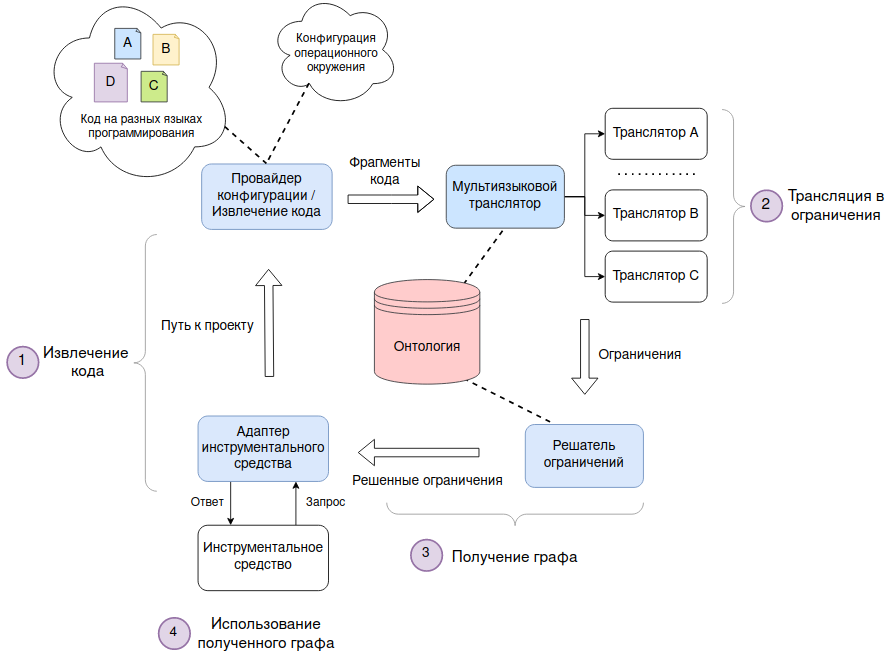
\includegraphics[height=0.85\textheight]{inc/img/framework}}
    \caption{Структура метода в виде диаграммы потока данных}
    \label{fig:framework}
\end{figure}

\section{Исследование средств реализации}

Учитывая поставленные задачи
логичным решением было выбрать популярный формат данных, который хорошо поддерживается современными
языками. В качестве основного формата передачи (т.е. носителем) ограничений решено было выбрать JSON.
Он является универсальным форматом структурированных данных, используемым в большом количестве
различных технологий и инструментов. В данном случае, формат был выбран по следующим причинам:
\begin{itemize}
    \item простота и универсальность,
    \item широкая поддержка в различных языках и средствах,
    \item относительная компактность,
    \item частая интеграция формата в существующих инструментальных средствах.
\end{itemize}

В целом язык не является основополагающим при разработке анализатора, так как не требуется
никаких специфических технологий для его реализации. При разработке в рамках данной работы
было решено выбрать язык Golang. Это прикладной императивный язык, поддерживающий
компиляцию в машинный код и небольшой рантайм, при этом сопровождая большинство
удобных функциональных возможностей для упрощения процесса разработки.
Из плюсов языка в контексте данного проекта можно отметить следующие особенности:
\begin{itemize}
    \item простота синтаксиса и семантики,
    \item наличие статической типизации,
    \item относительно легкая работа с динамическими (как JSON) данными,
    \item большое количество различных библиотек и очень высокое качество средств поддержки разработчика,
    \item быстрая компиляция и высокое быстродействие программ.
\end{itemize}

Минусами языка выступают: ограниченная система типов, слабая поддержка нетривиальных подходов к решению задач,
сильный расчет на динамические проверки во время исполнения.
Однако, для данного проекта эти минусы несущественны и не помешают реализации
основных модулей анализатора.
\clearpage
\chapter{Описание основных сценариев использования анализатора в сочетании с
инструментальными средствами программирования}

\section{Интеграция в различные инструментальные средства}

Анализатор, поставляющий информацию, описанную в \ref{constraints-desc} способен
поддерживать большое количество разнообразных инструментальных средств. Соответствующие
возможности анализатора отражены в таблице \ref{analysis-tooling}.

\begin{table}[h]
    \caption{Поддержка анализатором различных сценариев использования инструментальных средств}
    \resizebox{1 \textwidth}{!}{\begin{tabular}{|p{3cm}|p{3cm}|p{10cm}|}
    \hline Сценарий использования & Поддержка & Необходимая информация \\ 
    \hline Обнаружение багов & Частично & Идентификаторы; типы идентификаторов; значения идентификаторов; языкоспецифичная информация \\
    \hline Обнаружение уязвимостей & Отсутствует & Полная информация о системном окружении; знание уязвимостей различных библиотек и фреймворков \\
    \hline Соблюдение стиля кода и стандартов & Частично & Полный доступ к тексту и языкоспецифичному AST \\
    \hline Оценка сложности кода & Частично & Взаимосвязи различных идентификаторов, знание языкоспецифичных конструкций \\
    \hline Анализ зависимостей & Полностью & Идентификаторы и связи объявление-ссылка \\
    \hline
    \end{tabular}}\label{analysis-tooling}
\end{table}

Стоит подробнее описать каждый из сценариев для выявления возможностей предлагаемого метода.

Обнаружение багов может производиться на разных уровнях. Багом в данном случае может
считаться непреднамеренная функциональность (или её отсутствие), не отвечающая ожиданиям разработчика.
Соотвественно, в категорию багов, выявляемых анализатором могут потенциально входить:
неразрешенная ссылка, больше одной ссылки на определенный идентификатор, отсутствие ссылок
на определенный идентификатор. Баги иного рода находятся за рамками метода анализа, в первую
очередь из-за отсутствия возможности отслеживать значения идентификаторов, т.е.
отсутствие концепции \textit{переменной} или \textit{привязки}.

Обнаружение уязвимостей является довольно специфичным и сложным процессом, поэтому
количество сопровождаемой методом информации чаще всего будет недостаточным. Это связано
в первую очередь с отсутствием языкозависимой информации о типах или функциях, которые
могут содержать уязвимость. Соответственно, для реализации средств обнаружения уязвимостей в ПО
метод не подходит.

Соблюдение стиля кода и стандартов часто вовлекает идентификаторы. В контексте
анализа стиля назаваний переменных в проекте метода может быть достаточно. Однако, метод
не сопровождает никакой информации об исходном AST исходного языка, поэтому \textit{применение}
каких-либо рекомендаций по стилю может быть довольно сложным.

Оценка сложности кода вовлекает в себя использование различных метрик, например цикломатическая сложность
функции, связность классов или высота дерева наследования. Метод позволяет оценивать такие метрики как:
количество переменных в одной области видимости, связность на уровне модулей или файлов, количество
использований какого-либо определения. Оценка иных метрик сложна в первую очередь по причине отсутствия
языкоспецифичной информации.

Анализ зависимостей является важным процессом для обеспечения поддержки ПО. Рассматриваемый
метод анализа является в сущности способом построить граф объявлений и ссылок (или def-use граф), поэтому
для данного сценария использования он подходит очень хорошо. В сущности, метод позволяет обеспечивать
\textit{межъязыковой} анализ зависимостей, что может быть полезно в инструментах линтинга или
сбора статистики.

Таким образом, хоть поддержка различных инструментальных средств в контексте мультязыкового анализа и
ограничена, применимость метода всё еще довольно высока. Особенно это касается анализа зависимостей
в проекте. Основной особенностью метода является стирание языкоспецифичной информации, что
сильно уменьшает количество возможных сценариев использования, но в контексте некоторых сценариев использования
это не требуется. Одним из таких сценариев является поддержка разработчика в процессе кодирования.

\section{Реализация LSP как одного из сценариев интеграции метода}

В данной работе в качестве основного примера интеграции метода анализа было решено реализовать
анализатор, совместимый с LSP \Abbrev{LSP}{language server protocol --- протокол языкового сервера}
 \cite{LSP-spec}. LSP является протоколом, обобщающим языковые концепции для получения общих
методов взаимодействия с программой в контексте инструментальных средств разработки (в первую очередь IDE).

В возможные сценарии LSP (обобщенно) входит:
\begin{enumerate}[1)]
    \item найти объявление или определение идентификатора (типа или терма),
    \item определить иерархию вызовов,
    \item найти все ссылки на идентификатор,
    \item построить иерархию вызовов/наследования,
    \item подсветить идентификатор под курсором,
    \item автодополнение идентификатора под курсором,
    \item дать подсказку по проблеме под курсором (Inlay hint),
    \item остальные функции связанные с редактированием (подсветка, форматирование).
\end{enumerate}


В таблице \ref{lsp_functionality} представленно разделение приведенных сценариев на основе необходимой для анализа информации.
\begin{table}[H]
    \caption{Разделение сценариев по требуемой информации}\label{lsp_functionality}
    \begin{tabular}{|p{5.0cm}|p{5.0cm}|p{5.0cm}|}
    \hline Сценарий & Назначение & Необходимая информация \\
    \hline Поиск объявления или определения & Навигация по коду & Информация о областях видимости; информация о типах \\
    \hline Определение иерархии вызовов & Навигация по коду & Информация о областях видимости; информация о типах \\
    \hline Поиск ссылок на идентификатор & Навигация, редактирование & Информация о областях видимости; информация о типах \\
    \hline Подсветка символа & Редактирование & Информация о областях видимости \\
    \hline Автодополнение символа & Редактирование & Информация о областях видимости; информация о типах \\
    \hline Подсказка по проблеме & Редактирование, корректность & Специфическая для языка информация \\
    \hline
    \end{tabular}
\end{table}

Как видно из таблицы, даже при таком грубом разделении сценариев, описываемый метод способен поддержать подавляющее
большинство сценариев LSP. В теории, возможно создание \textit{универсального LSP анализатора}, позволяющего вовлекать не только
языкоспецифичный анализ, но и межъязыковой. Такой анализатор будет иметь возможность сопровождать приведенные сценарии использования
для любого количества языков и их комбинации, что может позволить сильно увеличить продуктивность разработчиков в отношении
разработки и поддержки ПО.

\clearpage
\chapter{Программная реализация анализатора и инфраструктуры}

Данная реализация анализатора является первичной и её главная задача это иллюстрация работоспособности метода анализа.
Поэтому данный анализатор включает дополнительную инфраструктуру, не рассматриваемую в методе. Такие компоненты
анализатора будут отмечены соответствующим примечанием в тексте.

\section{Общая архитектура}

\subsection{Структура анализатора}

Исходя из раздела \ref{sec:architecture} анализатор, реализующий описываемый метод мультиязыкового анализа будет включать в себя следующие
компоненты:
\begin{enumerate}[1)]
    \item провайдер конфигурации и кода,
    \item мультиязыковой транслятор,
    \item решатель ограничений,
    \item адаптер для конкретного инструментального средства (в данном случае LSP сервера).
\end{enumerate}

% Plantuml?
% TODO: Диаграмма компонентов
% TODO: Общая диаграмма деятельности (общий пайплайн)

\subsection{Реализация онтологии}

\section{Провайдер конфигурации и кода}

\section{Мультиязыковой транслятор}

\section{Решатель ограничений}

\section{Адаптер инструментального средства}

% TODO: Протокол анализатора
% TODO: Кэш компонентов
\chapter{Оценка показателей анализатора на избранных тестовых проектах}

Для оценки анализатора (а также в первую очередь метода анализа) было создано три тестовых проекта.
Проекты были созданы исходя из следующих критериев:
\begin{itemize}
    \item использование нескольких популярных языков в одном проекте,
    \item каждый проект решает задачу в определенной уникальной предметной области,
    \item используемые языки должны представлять различные парадигмы программирования,
    \item каждый из проектов должен вовлекать различные сценарии использования LSP.
\end{itemize}

Все полученные ограничения находятся в открытом репозитории проекта в виде файлов кода на языке TypeScript. \footnote{https://github.com/UberDever/crosslingual-analysis/tree/master/projects/crossy/lsp-adapter/examples}

\section{Пример 1 -- C\# и Visual Basic}

\subsection{Общее описание}

Приложение, реализованное на C\# использует слой взаимодействия на уровне байткода IL и имеет в зависимостях библиотеку,
реализованную на Visual Basic. Весь проект объединен через Solution файл. Такой сценарий часто встречается
в legacy приложениях, при переходе кодовой базы с Visual Basic на C\#.

Вовлекаемые языки: C\#, Visual Basic, XML (\texttt{.sln}, \texttt{.vbproj} и \texttt{.csproj} файлы).
Предположительные предметные области: Энтерпрайз приложения, частные коммерческие решения.
Рассмотренные парадигмы языков: ООП, структурированные данные.

\subsection{Окружение}

При извлечении кода могут быть использованы файлы проектов \texttt{.vbproj} и \texttt{.csproj}, в дальнейшей
достаточно построение <<слепка>> файловой структуры проекта.

\subsection{Трансляция и решение}

Трансляция может вовлекать в себя стандартный reaching definition анализ \cite{static-program-analysis} и прямое отображение
статической структуры классов и объектов на ограничения графов областей. При отображении не были использованы
структурные предикаты, так как структура модулей и классов C\# не имеет определенной семантики в отношении
типов и возможной вложенности. 

\subsection{Онтология}

Типы, добавленные в онтологию:
\begin{itemize}
    \item \texttt{Integer} -- целочисленное число неспецифицированной точности,
    \item \texttt{Top} -- супертип всех возможных типов, также является маркером отсутствия информации об идентификаторе.
\end{itemize}

\subsection{Сценарии LSP}

Для данного примера было решено реализовать два сценария использования, характерных для ООП языков: <<Type hierarchy>> 
(получение иерархии типов) и <<Go to definition/declaration>> (перейти к объявлению/использованию).
Предполагаемые примеры внешнего вида реализации таких сценариев показаны на рисунке \ref{fig:typehierarchy} и рисунке \ref{fig:gotodef}
соответственно.


\section{Пример 2 -- С++, Python 3 и Shell}

\section{Пример 3 -- Golang и JavaScript}

% TODO: 3 примера, 6 сценариев.
% Проект (описание, области, языки, парадигмы) -> необходимое/использованное окружение -> особенности трансляции -> ограничения -> подстановка -> скрины
\clearpage

\backmatter %% Здесь заканчивается нумерованная часть документа и начинаются ссылки и
            
%% \Conclusion % заключение к отчёту

В результате данной работы было выполнено исследование существующих методов мультязыкового анализа,
выявлены их достоинства и недостатки. Проанализированы существующие инструменты поддержки разработчика,
поддерживающие анализ множества языков и их связей.

Был разработан метод мультиязыкового статического анализа, позволяющий
обеспечить инструментальные средства поддержки разработчика. Данный метод отвечает требованиям
к гибкости и языконезависимости, а также к корректности семантических свойств используемого представления.

Также, для подтверждения работоспособности данного метода был разработан мультиязыковой анализатор
и адаптер избранного инструментального средства (сервера LSP). В ходе разработки были созданы
протокол и онтология, вместе позволяющие обеспечивать согласованность мультиязыковых фрагментов
кода. Была произведена тестовая интеграция сервера LSP в IDE Visual Studio Code с демонстрацией определенных
сценариев использования LSP.

Задачи выпускной квалификационной работы выполнены в полном объеме, поставленная цель достигнута.

%%% Local Variables: 
%%% mode: latex
%%% TeX-master: "rpz"
%%% End: 
%% заключение


% % Список литературы при помощи BibTeX
% Юзать так:
%
% pdflatex rpz
% bibtex rpz
% pdflatex rpz

\bibliographystyle{ugost2008}
\bibliography{rpz}

%%% Local Variables: 
%%% mode: latex
%%% TeX-master: "rpz"
%%% End: 



\appendix   % Тут идут приложения

\chapter{Протоколы мультиязыкового анализатора}
\label{cha:appendix1}

% TODO: Протоколы
\begin{minted}[linenos=true]{ts}
    const a: 1 | "a" = 1
    const b: 1 | "a" = "a"
    const c: 1 | "a" = true
\end{minted}

%%% Local Variables: 
%%% mode: latex
%%% TeX-master: "rpz"
%%% End: 


\include{91-appendix2}

\end{document}

%%% Local Variables:
%%% mode: latex
%%% TeX-master: t
%%% End:
